Der  LT3741  ist  sowohl   Spannungsgesteuert   wie   auch  Stromgesteuert.  Der
Spannungsteiler  $R_{11} \parallel R_2$ (siehe Abbildung  \ref{fig:circuit:buck}
oder    Abbildung    \ref{fig:circuit:buck:uset})   erlaubt   das   Messen   der
Ausgangsspannung  und  ein  Shunt-Widerstand  $R_4$   erm\"oglicht   die  genaue
\"Uberwachung des Stromes durch die Spule  $L_1$.  Der Widerstand $R_4$ wurde so
gew\"ahlt damit der  maximale  Ausgangsstrom  maximal  \SI{5}{\ampere}  betragen
kann.

Strom\"uberwachung   ist  sehr  wichtig  bei  einer  solchen  Aufgabe   wo   die
Ausgangsspannung  sich  konstant  \"andert.  Sie erlaubt  genauer  vorhersebares
Verhalten der Spannungs\"anderung am Ausgang -- \"Uberschiessen der Sollspannung
und  extreme  Stromspitzen  in  der  Spule  k\"onnen  besser  vermieden  werden.

Weiter   kann   ein   Stromgesteuerter   Regler  auch  als   Konstantstromquelle
funktionieren. Diese Eigenschaft  ist  vorallem  dann  von  Bedeutung  wenn  der
Arbeitspunkt  sich  im  ``steilen''  bereich  der   UI-Kennlinie  des  PV-Moduls
befindet.

Die  Feedback-Widerst\"ande   $R_2$   und   $R_{11}$   wurden  nach  der  Formel
\ref{eq:circuit:buck:feedback_resistors}       dimensioniert      damit      die
Ausgangsspannung maximal \SI{23}{\volt} betr\"agt.

\begin{equation}
    U_{out} = \SI{1.21}{\volt} \left( 1 + \frac{R_{11}}{R_2} \right)
    \label{eq:circuit:buck:feedback_resistors}
\end{equation}

Die Ausgangsspannung kann  danach  durch Anheben der Bezugsspannung $BUCK\_USET$
nach der  Formel \ref{eq:circuit:buck:uset} ver\"andert werden. 

\begin{equation}
    U_{out} = (\SI{1.21}{\volt} - BUCK\_USET) \cdot \frac{R_{11} + R_2}{R_2}
    \label{eq:circuit:buck:uset}
\end{equation}

Wobei $BUCK\_USET$ die analoge Spannung vom  ersten  DAC  ist.  In der Abbildung
\ref{fig:circuit:buck:uset} ist die dazugeh\"orige Schaltung.

\begin{figure}[th!]
    \center
    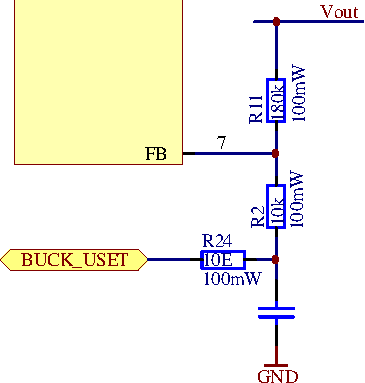
\includegraphics[width=.35\textwidth]{images/circuit/buck-uset.pdf}
    \caption{Einstellung der Ausgangsspannung durch \"Anderung der Bezugsspannung im Feedback-Loop mittels einer analogen Steuerspannung von 0V bis 1.21V}
    \label{fig:circuit:buck:uset}
\end{figure}

Analog zur Ausgangsspannung kann auch der Maximalstrom eingestellt werden. Durch
anlegen einer  analogen  Spannung  zwischen \SI{0}{\volt} und \SI{1.5}{\volt} am
Eingang  CTRL1 des LT3741 kann  direkt  der  maximale  \emph{Durchschnittsstrom}
durch die Spule $L_1$ und  somit  der maximale Ausgangsstrom eingestellt werden.

\begin{figure}[th!]
    \center
    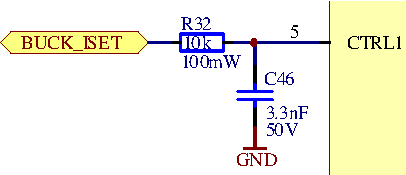
\includegraphics[width=.4\textwidth]{images/circuit/buck-iset.pdf}
    \caption{Einstellung des Maximalstroms mittels einer analogen Steuerspannung von 0V bis 1.5V}
    \label{fig:circuit:buck:iset}
\end{figure}

Die Abbildung \ref{fig:circuit:buck:iset} zeigt  die  dazugeh\"orige  Schaltung.
Der   maximale  durchschnittliche  Ausgangsstrom  $I_o$  wird  mit  der   Formel
\ref{eq:circuit:buck:output_current} berechnet

\begin{equation}
    I_o = \frac{U_{CTRL1}}{30 \cdot R_4}
    \label{eq:circuit:buck:output_current}
\end{equation}

wobei $U_{CTRL1}$ die  analoge  Steuerspannung vom zweiten DAC ist und $R_4$ der
\SI{10}{\milli\ohm}    Shunt-Widerstand    ist,   welcher   in   der   Abbildung
\ref{fig:circuit:buck} zu sehen ist.

Damit der Mikrocontroller angemessene Steuerspannungen  generieren kann, braucht
er die Ausgangsspannung und den Ausgangsstrom zu messen.

Die   Ausgangsspannung   wird   mittels   der   Schaltung   in   der   Abbildung
\ref{fig:circuit:buck:umeas} gemessen. Die Widerst\"ande $R_{12}$  und  $R_{15}$
wurden  so  dimensioniert  damit  die  Spannung  $BUCK\_UMEAS$  im  Bereich  von
\SI{0}{\volt} bis \SI{1.5}{\volt} skaliert ist.

\begin{figure}[th!]
    \center
    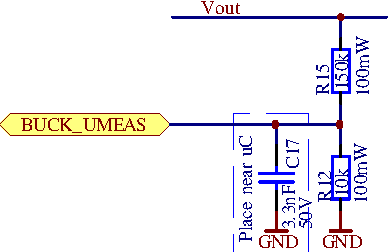
\includegraphics[width=.45\textwidth]{images/circuit/buck-umeas.pdf}
    \caption{Messen der Ausgangsspannung}
    \label{fig:circuit:buck:umeas}
\end{figure}

Der  Ausgangsstrom  wird  mittels  einem  Shunt-Widerstand  $R_5$  differentiell
gemessen.  Die  Schaltung dazu ist in der Abbildung \ref{fig:circuit:buck:imeas}
dargestellt.

\begin{figure}[th!]
    \center
    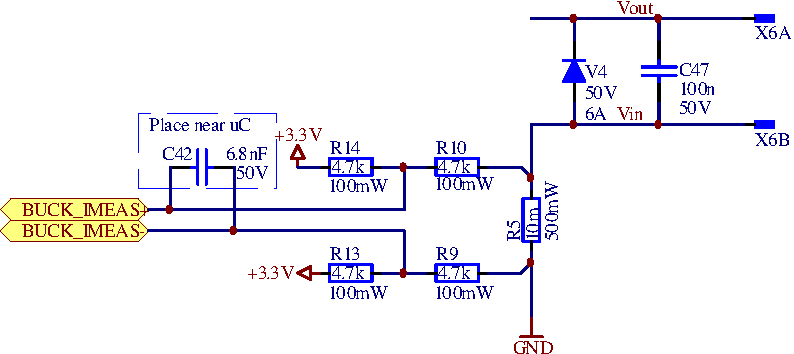
\includegraphics[width=.85\textwidth]{images/circuit/buck-imeas.pdf}
    \caption{Messen des Ausgangsstromes}
    \label{fig:circuit:buck:imeas}
\end{figure}

Es  ist  zu  beachten,  dass  die  Widerst\"ande  $R_{10}$  und  $R_{14}$  einen
Bias-Strom durch den Widerstand $R_5$  verursachen.  Somit  entsteht ein kleiner
Spannungs-Offset.
\begin{equation}
    U_{offset} = \frac{ \SI{3.3}{\volt} \cdot R_5 }{ R_{14} + R_{10} + R_5 }
    \label{eq:circuit:buck:shunt_offset}
\end{equation}

Da   der   ADC   eine   12-bit   Aufl\"osung   mit  einer  Referenzspannung  von
\SI{3.3}{\volt} hat, gilt:
\begin{equation}
    U_{step} = \frac{\SI{3.3}{\volt}}{2^{12}} = \SI{806}{\micro\volt}
    \label{eq:circuit:buck:adc_step}
\end{equation}

Die Widerst\"ande $R_9$, $R_{10}$, $R_{10}$ und  $R_{14}$  sollten  so klein wie
m\"oglich  dimensioniert  werden damit St\"orungen an  den  Leitungen  minimiert
werden  k\"onnen,  aber  sollten immer noch gross genug sein, damit  $U_{offset}
\leq  U_{step}$.  Zu  gross  d\"urfen  sie  auch  nicht  sein,  weil  sonst  die
Holding-Time  des   ADCs   nicht   mehr   erf\"ullt   ist  (was  bei  ca.  $\geq
\SI{5}{\kilo\ohm}$      der      Fall     ist).     Aus     den      Gleichungen
\ref{eq:circuit:buck:shunt_offset} und \ref{eq:circuit:buck:adc_step} kann jetzt
nach den 4 Widerst\"anden aufgel\"ost werden. Es gilt:
\begin{align*}
                          U_{step} &\geq U_{offset} \\
    \frac{\SI{3.3}{\volt}}{2^{12}} &\geq \SI{3.3}{\volt} \cdot \frac{R_5}{R_x + R_5} \\
                  \frac{1}{2^{12}} &\geq \frac{R_5}{R_x + R_5} \\
                               R_x &\geq \left( 2^{12} - 1 \right) \cdot R_5 \\
\end{align*}

wobei  $\frac{R_x}{2}  =  R_{9}  =  R_{10} = R_{13} = R_{14}$. Berechnet  ergibt
$\frac{R_x}{2} \approx \SI{22}{\ohm}$.

Eine weitere Einschr\"ankung, vorallem bei  kleinen  Widerst\"anden,  ist,  dass
nicht  unn\"otig  viel  Leistung  verbraten  werden sollte. Deshalb  werden  die
Widerst\"ande ein wenig h\"oher mit \SI{270}{\ohm} dimensioniert. In diesem Fall
ist der Leistungsverlust aller 4 Widerst\"ande:
\begin{equation*}
    P_{loss} \approx \frac{\SI{3.3}{\volt}^2}{2\cdot \SI{270}{\ohm}} \approx \SI{20}{\milli\watt}
\end{equation*}

Die gemessene Spannung  am  Shunt-Widerstand  ist recht klein. Deshalb verwenden
wir  den  im  Mikrocontroller  eingebauten  vorverst\"arker  (PGA),   was   eine
Verst\"arkung von bis  zu Faktor 64 erreichen kann. Das verst\"arkte Signal wird
intern an der eingebauten differentiellen ADC weitergeleitet.

